\chapter{Analisi delle librerie per la visualizzazione di mappe web}

\section{Introduzione}
Le mappe web interattive sono diventate strumenti fondamentali per la visualizzazione e l'analisi di dati geospaziali in ambito scientifico, industriale e ambientale. Con la crescente disponibilità di dataset georeferenziati di grandi dimensioni, la necessità di soluzioni web performanti e flessibili per la loro rappresentazione è oggi più sentita che mai. Negli ultimi anni, lo sviluppo di numerose librerie JavaScript ha reso possibile integrare con relativa facilità mappe interattive all'interno di applicazioni web, offrendo funzionalità avanzate sia per la visualizzazione 2D che 3D.

In particolare, il caso d'uso affrontato in questo lavoro, ossia la rappresentazione di oltre 100.000 punti geolocalizzati, ciascuno associato a un valore di intensità del rumore subacqueo, pone una sfida significativa in termini di rendering e interattività. L'obiettivo principale di questo capitolo è analizzare lo stato dell'arte delle principali librerie JavaScript per la visualizzazione di mappe, con un focus su quelle in grado di gestire grandi volumi di dati mantenendo buone performance grazie al supporto a tecnologie come WebGL \cite{mapbox-gl-js}.

Verranno confrontate le soluzioni più diffuse, sia \textit{open-source} che commerciali, valutandone la modularità, la facilità d'integrazione, e la capacità di offrire un'esperienza utente fluida anche in scenari complessi. Il fine ultimo è individuare la libreria più adatta a essere integrata nel sistema M-NAT, garantendo un'interfaccia reattiva, scalabile e in grado di restituire in modo chiaro e immediato l'informazione acustica elaborata dal modello.

\subsection{Cos'è un Heatmap}
Una \emph{heatmap} è una rappresentazione grafica bidimensionale che utilizza una scala cromatica per visualizzare l'intensità o la concentrazione di un fenomeno all'interno di una griglia o mappa. Le tonalità più calde (es. rosso, arancione) indicano valori più elevati, mentre quelle fredde (es. blu, verde) rappresentano valori più bassi.

Questo tipo di visualizzazione facilita l'individuazione immediata di pattern, cluster o anomalie in insiemi di dati complessi, risultando particolarmente utile in ambiti come l'analisi geospaziale, il web analytics, l'urbanistica, l'economia e la ricerca scientifica. In applicazioni geospaziali, una \emph{spatial heatmap} sovrappone dati di densità geolocalizzata su una mappa, evidenziando visivamente le aree di maggiore concentrazione del fenomeno studiato \cite{vwo-heatmap,heatmap-wikipedia,clarity-heatmap}.


\section{Criteri di valutazione}
Per confrontare le diverse librerie sono stati definiti alcuni criteri fondamentali:
\begin{itemize}
  \item \textbf{Facilità d'integrazione e documentazione}
  \item \textbf{Performance e fluidità dell'interazione}
  \item \textbf{Supporto a dati vettoriali e raster}
  \item \textbf{Licenza e costi d'uso}
  \item \textbf{Compatibilità con altri strumenti e framework}
\end{itemize}

% import leaflet.tex
\section{Leaflet}
\label{ch:leaflet}

\subsection{Facilità d'integrazione e documentazione}  
Leaflet fornisce una guida introduttiva, esempi interattivi e un'API reference completa sul sito ufficiale \cite{leaflet-doc}.  
La curva di apprendimento è bassa grazie a metodi semplici come \texttt{L.map()}, \texttt{L.tileLayer()} e \texttt{L.marker()}, e la comunità mantiene un ampio catalogo di plugin per estendere ogni funzionalità, dal \textit{clustering} dei marker all'integrazione con dataset GeoJSON complessi \cite{react-leaflet}.

\subsection{Performance e fluidità dell'interazione}  
Di default Leaflet usa SVG e elementi DOM per il rendering, garantendo ottime performance fino a 5.000–10.000 feature\cite{supercluster}.  
Per dataset più voluminosi, plugin come \texttt{Supercluster} permettono di raggruppare i punti via \textit{clustering} su struttura R‑tree e riducono drasticamente i marker renderizzati\cite{supercluster}.  
In alternativa, estensioni WebGL come \texttt{leafgl} sfruttano la GPU per mantenere un'interattività fluida anche con decine di migliaia di feature\cite{leafgl}.  

WebGL (Web Graphics Library) è un'API JavaScript per il rendering di grafica 2D e 3D interattiva ad alte prestazioni direttamente nel browser, sfruttando l'accelerazione hardware della GPU \cite{wiki-webgl}.  
Avere supporto a WebGL all'interno di una libreria per mappe web è fondamentale per gestire grandi quantità di dati geospaziali e garantire un'esperienza utente fluida, poiché il carico grafico viene trasferito dalla CPU alla GPU tramite \textit{shader} e buffer dedicati \cite{khronos-webgl}.  
Senza WebGL, il rendering di dataset massivi ricadrebbe sul DOM e sulla CPU, con evidenti rallentamenti e limiti di scala.


\subsection{Supporto a dati vettoriali e raster}  

I \textit{raster} sono un modello di dati spaziali in cui lo spazio geografico viene suddiviso in una griglia regolare di celle (o pixel), organizzate in righe e colonne, e ciascuna cella contiene un valore numerico che rappresenta un fenomeno reale, come temperatura o elevazione. Questi dati derivano spesso da immagini digitali, fotografie aeree, satellitari o mappe scannerizzate, e sono particolarmente adatti a rappresentare variabili continue distribuite su un'area. \cite{esri-raster-model,qgis-raster-data}

La gestione dei \emph{raster tiles} (p.es. OpenStreetMap o MapTiler) è immediata con \texttt{L.tileLayer()}\cite{maptiler-raster}.  
Il supporto ai \emph{vector tiles} non è nativo, ma può essere aggiunto tramite plugin consolidati come \texttt{leaflet-geojson-vt} e \texttt{Leaflet.VectorGrid}, che frammentano i grandi file GeoJSON/TopoJSON in tile \textit{client‑side} per un caricamento e un clipping più efficienti \cite{leaflet-geojson-vt,vectorgrid}.  

\subsection{Licenza e costi d'uso}  
Leaflet è rilasciato sotto licenza BSD2‑Clause (Simplified) e BSD3‑Clause, entrambe estremamente permissive e compatibili con progetti commerciali senza obblighi di royalty.
Non esistono canoni d'uso; per chi desidera supporto professionale, sono disponibili piani di consulenza e SLA a pagamento offerti da terze parti. \cite{leaflet-doc, leaflet-license}

\subsection{Compatibilità con altri strumenti e framework}  
Viene concepita inizialmente come libreria JavaScript; per React esiste \texttt{ReactLeaflet}, una raccolta di componenti che incapsulano mappe Leaflet in JSX e ne semplificano l'uso all'interno di applicazioni React. \cite{react-leaflet}

\newpage
\section{Mapbox GL}
\label{ch:mapbox}

\subsection{Facilità d'integrazione e documentazione}  
Mapbox GL JS è una libreria JavaScript client-side che sfrutta WebGL per costruire mappe interattive direttamente nel browser.  
La documentazione ufficiale è organizzata in guide passo‑passo e in una API reference dettagliata, entrambe mantenute costantemente aggiornate sul sito Mapbox.  
L'installazione può avvenire tramite CDN o, per un'integrazione nei workflow moderni, installando il pacchetto \texttt{mapbox-gl} con npm o yarn. \cite{mapbox-docs}  

\subsection{Performance e fluidità dell'interazione}  
Grazie al rendering GPU‑accelerato, Mapbox GL JS è in grado di mantenere un frame rate elevato anche con centinaia di migliaia di feature.
Le metriche principali per misurare le prestazioni sono il \emph{render time}, il \emph{source update time} e il \emph{layer update time}, tutte analizzabili tramite logging interno.  
Per dataset estremamente grandi è possibile ottimizzare i tileset applicando tecniche di \emph{tile clipping} e caching client-side, come descritto nella guida ufficiale ai \textit{vector tiles} \cite{mapbox-vector, article-highperf}.  

\subsection{Supporto a dati vettoriali e raster}  
Mapbox GL JS supporta nativamente i \emph{vector tiles} in formato MVT, uno standard basato su Google Protobuf per file con estensione \texttt{.mvt}\cite{mapbox-vector}.  
Il caricamento di \emph{raster tiles} da terze parti è altrettanto semplice: basta definire una sorgente di tipo \texttt{raster} e aggiungere il layer corrispondente, seguendo gli esempi forniti nella documentazione \cite{mapbox-raster}.  

\subsection{Licenza e costi d'uso}  
A partire dalla versione 2, Mapbox GL JS è distribuito sotto licenza commerciale e richiede un \textit{token} Mapbox per l'uso in produzione.  
Il modello di pricing è basato sui \emph{map loads} mensili, con una soglia gratuita di base e piani a consumo che scalano automaticamente con l'utilizzo \cite{mapbox-license-v2, mapbox-pricing}.  

\subsection{Compatibilità con altri strumenti e framework}  
In ambito React è disponibile \texttt{react-map-gl}, una raccolta di componenti che semplifica l'integrazione di Mapbox GL JS in applicazioni basate su React \cite{react-map-gl,mapbox-react-tutorial}.  

Per analisi spaziali avanzate è possibile combinare Mapbox GL JS con librerie come Turf.js, aggiungendo operazioni geospaziali direttamente sul client.  
Chi volesse implementare visualizzazioni 3D o modelli personalizzati può estendere la mappa con Three.js tramite un CustomLayer.  
Infine, Mapbox offre SDK nativi per iOS e Android, che permettono di riutilizzare stili e tileset MVT nelle applicazioni mobile con API coerenti \cite{mapbox-ios, mapbox-mobile-sdk}.  

\newpage
\section{Deck.gl}
\label{ch:deckgl}

\subsection{Facilità d'integrazione e documentazione}  
Deck.gl è un framework GPU‑powered pensato per la visual exploratory data analysis di grandi dataset geospaziali.  
La documentazione ufficiale, disponibile sul sito di Deck.gl (https://deck.gl/docs), include un'introduzione, guide passo‑passo e una API reference completa, oltre a esempi di codice e uno showcase interattivo \cite{deckgl-docs}.  
L'installazione è semplice: basta aggiungere il pacchetto \texttt{deck.gl} da npm o yarn, oppure includere i bundle via CDN \cite{deckgl-npm,deckgl-github}.  

\subsection{Performance e fluidità dell'interazione}  
Grazie al rendering WebGL2 (e supporto sperimentale a WebGPU), Deck.gl mantiene frame rate elevati anche con milioni di punti: per esempio, lo \texttt{ScatterplotLayer} rimane fluido fino a circa 1M di elementi su hardware consumer, degradando in modo controllato oltre i 10M \cite{deckgl-performance}.  
Demo storiche mostrano la visualizzazione di oltre 2M di punti e 36K viaggi in tempo reale con interpolazione GPU di New York City \cite{deckgl-uber-blog}.  
Il core di Deck.gl è ottimizzato per il caricamento e l'aggiornamento dei dati a livello di tile, riducendo la pressione sulla CPU e sfruttando in modo efficiente la GPU \cite{deckgl-github}.  

\subsection{Supporto a dati vettoriali e raster}  
Deck.gl offre una vasta libreria di layer per dati vettoriali; fra i più rilevanti abbiamo: 

\begin{itemize}
    \item \texttt{GeoJsonLayer},
    \item \texttt{MVTLayer}
    \item \texttt{VectorTileLayer}
\end{itemize}

Queste librerie consentono di caricare GeoJSON e Mapbox Vector Tiles in MVT con clipping e streaming dinamico\cite{deckgl-vector,deckgl-mvtlayer}.  
Per i raster tiles, il plugin \texttt{deck.gl-raster} e il layer \texttt{RasterTileLayer} (in Carto integration) permettono di visualizzare immagini satellitari o DEM con WebGL direttamente nel canvas di Deck.gl.  
L'architettura a layer composabili facilita anche l'estensione a casi d'uso personalizzati, integrando WebGL modules per elaborazioni \textit{on-the-fly} di dati raster avanzati\cite{deckgl-maptiler,deckgl-raster-plugin}.  

\subsection{Licenza e costi d'uso}  
Deck.gl è rilasciato con licenza permissiva MIT, che ne consente l'uso, la modifica e la ridistribuzione anche in progetti commerciali senza royalty. \cite{deckgl-license}  
Non ci sono costi di licenza; l'unico requisito è l'attribuzione del copyright e la preservazione del testo di licenza originale.  

\subsection{Compatibilità con altri strumenti e framework}  
Deck.gl offre una buona integrazione con React tramite il componente \texttt{@deck.gl/react}, che espone \texttt{DeckGL} e hooks per gestire view state e interazioni in JSX. \cite{deckgl-react}  
Per altri framework, la comunità mantiene binding e plugin non ufficiali (ad es. Vue, Angular) raccolti in \texttt{deck.gl-community}, benché con supporto meno costante. \cite{deckgl-community}
Il layer system di Deck.gl è inoltre progettato per lavorare insieme a librerie di analisi spaziale come Turf.js e a motori di rendering 3D come Three.js attraverso CustomLayer. cite{deckgl-faq}

\newpage
\section{OpenLayers}
\label{ch:openlayers}

\subsection{Facilità d'integrazione e documentazione}
OpenLayers mette a disposizione una documentazione ufficiale molto dettagliata, con guide introduttive, esempi interattivi e API reference sul sito del progetto \cite{openlayers-doc}.  
Il codice sorgente e il tracker delle issue sono ospitati su GitHub, dove si trova anche il file di licenza Clear BSD 2‑Clause.
È inoltre attivo un ecosistema di wrapper e plugin non ufficiali raccolti in repository quali \say{awesome-openlayers} \cite{openlayers-github,awesome-openlayers}.

\subsection{Performance e fluidità dell'interazione}
Il supporto WebGL in OpenLayers permette di sfruttare la GPU per il rendering di geometrie complesse: esempi ufficiali mostrano come il layer \texttt{WebGLVectorLayer} mantenga un frame rate elevato anche con decine di migliaia di punti. \cite{openlayers-webgl-example} 
Workshop dedicati illustrano tecniche di ottimizzazione, come il tiling client‑side e la gestione dinamica dei dati, per mantenere interactive performance anche in scenari di grandi dataset.
Discutere problemi di performance su forum come GIS StackExchange rivela strategie quali clustering e buffer dinamici per ridurre il carico di rendering. \cite{openlayers-webgl-workshop,openlayers-issue-perf}

\subsection{Supporto a dati vettoriali e raster}
\subsubsection*{Vector tiles}
OpenLayers supporta nativamente Mapbox Vector Tiles (MVT) tramite il layer \texttt{VectorTileLayer}, consentendo styling lato client e caricamento tile‑by‑tile.
Sono disponibili esempi per OSM Vector Tiles che utilizzano il formato MVT per ottenere ottime prestazioni con dataset di medie dimensioni. \cite{openlayers-mapbox-vector-tiles,openlayers-osm-vector-tiles}

\subsubsection*{Raster tiles}
Il framework gestisce tile raster da sorgenti XYZ e WMS con le classi 

\begin{itemize}
    \item \texttt{ol/source/XYZ} 
    \item \texttt{ol/source/TileWMS}
\end{itemize}

semplificando l'uso di basemap come OpenStreetMap o servizi Geoserver\cite{openlayers-raster-xyz}.  
Per casi avanzati, la documentazione ufficiale risulta un'importante risorsa per ottenere più informazioni sulla riproiezione dei raster.

\subsection{Supporto a WebGL}
Il motore WebGL di OpenLayers, accessibile tramite \texttt{WebGLPointsLayer} e \texttt{WebGLVectorLayer}, sfrutta buffer di vertici e shader GLSL per trasferire gran parte del lavoro di rendering alla GPU, rendendo possibile la visualizzazione di grandi moli di dati con animazioni fluide. \cite{openlayers-webgl-example,openlayers-webgl-workshop}

\subsection{Licenza e costi d'uso}
OpenLayers è rilasciato sotto licenza Clear BSD 2‑Clause, una licenza permissiva che permette uso, modifica e ridistribuzione anche in progetti commerciali senza royalty \cite{openlayers-github,ol-cesium-license}.  
Non sono previsti costi di licenza, ma il progetto invita a donare tramite OSGeo per sostenere il mantenimento del software \cite{openlayers-doc}.

\subsection{Compatibilità con altri strumenti e framework}
Oltre a React, la comunità ha sviluppato binding per Vue, Angular e GWT, elencati nella pagina \say{Useful 3rd party libraries} del sito ufficiale.  
Per analisi spaziale lato client è comune integrare OpenLayers con Turf.js, come mostrato nell'esempio ufficiale \say{\texttt{turf.js}} \cite{awesome-openlayers,openlayers-turf-example}.  

\newpage
\section{Folium}
\label{ch:folium}

\subsection{Facilità d'integrazione e documentazione}  
Folium è una libreria Python che semplifica la creazione di mappe interattive basate su Leaflet direttamente da notebook e applicazioni web \cite{folium-doc}.
La documentazione ufficiale comprende un User Guide con esempi passo‑passo e un'\textit{API Reference} dettagliata, entrambi disponibili sul sito del progetto \cite{folium-userguide}.  
Il \textit{repository} GitHub ospita codice, issue e un elenco di plugin e pacchetti correlati (\textit{xyzservices}, streamlit‑folium) che estendono le funzionalità di base \cite{folium-github,folium-pypistats}.  
Online è facile reperire delle guide pratiche per integrare Folium in workflow di \textit{data science} basati, per esempio, su Jupyter Notebook \cite{folium-tutorial,folium-realpython}.

\subsection{Performance e fluidità dell'interazione}  
Di default Folium rende le feature come oggetti JavaScript nel DOM di Leaflet: ciò è efficiente per qualche migliaio di marker, ma può diventare lento con dataset superiori a 10.000 punti, come evidenziato da una discussione su StackOverflow riguardo al MarkerCluster, dove, per dataset molto voluminosi, viene consigliato di preprocessare i dati in vector tiles o di applicare tecniche di clustering lato server \cite{folium-cluster-issue}.  

Sono disponibili diversi plugin come \textit{MarkerCluster} e \textit{FastMarkerCluster}, mirati a migliorare l'esperienza utente con il crescere della dimensione del dataset \cite{folium-cluster-issue,folium-pypistats}.  
Il numero di download settimanali (più di 500.000) testimonia la diffusione di Folium e la necessità di \textit{best practice} per gestire prestazioni e scalabilità.

\subsection{Supporto a dati vettoriali e raster}  
Folium supporta nativamente diversi tipi di layer vettoriali (GeoJSON, Choropleth, HeatMap) e mette a disposizione \textit{convenience class} per aggiungere popup e tooltip dinamici.  
Il supporto a raster avviene tramite classi come \texttt{TileLayer}, \texttt{WmsTileLayer} e \texttt{ImageOverlay}, permettendo di utilizzare \textit{basemap} OpenStreetMap, mappe satellitari e overlay di immagini o video georeferenziati.  
Per esigenze avanzate di overlay raster in Jupyter, utilizzando \textit{Rasterio} è possibile integrare singole bande \textit{tiff} in mappe interattive. \cite{folium-raster,folium-tutorial, folium-doc}

\subsection{Licenza e costi d'uso}  
Folium è rilasciato sotto licenza MIT, liberamente utilizzabile, modificabile e ridistribuibile anche in contesti commerciali senza alcun costo di licenza.  
La gestione delle dipendenze e dei plugin avviene via PyPI, con aggiornamenti regolari e un ciclo di rilascio che segue le versioni di Leaflet sottostanti \cite{folium-lic,folium-pypi}.

\subsection{Compatibilità con altri strumenti e framework}  
Folium si integra con Jupyter Notebook e JupyterLab, generando mappe HTML \say{\textit{embeddate}} direttamente nelle celle del notebook.  
Esistono \textit{binding} pacchetti per far girare mappe Folium in applicazioni Streamlit (\texttt{streamlit-folium}) e wrapper per framework frontend come React, sebbene in questi casi si usino spesso \textit{iframe} o comunicazione via REST \cite{folium-github,folium-react}.  
L'ecosistema di plugin ospita esempi per l'uso con GeoPandas, Pandas e altri pacchetti di data science, facilitando l'integrazione in pipeline di elaborazione geospaziale \cite{folium-doc,folium-userguide}.

\newpage
\section{\textit{Benchmarking} Automatizzato per il Confronto Prestazionale tra Librerie}

Al fine di condurre un'analisi comparativa rigorosa e sistematica delle prestazioni offerte dalle diverse librerie di visualizzazione cartografica prese in esame, è stato realizzato un progetto separato il quale implementa una specifica funzionalità di benchmarking automatizzato. Questo sistema è stato impiegato per acquisire misurazioni quantitative e ripetibili dei tempi di esecuzione e rendering, minimizzando al contempo l'intervento manuale e le potenziali distorsioni da esso derivanti. Si è posta particolare enfasi nel garantire che ogni singola prova venisse eseguita in condizioni operative il più possibile isolate e \say{pulite}, ovvero esenti da interferenze dovute a stati precedenti dell'applicazione o a risorse memorizzate nella cache.
Grazie a tali dati, è stato possibile valutare la reattività di ogni libreria considerata e presentare, in questo elaborato, un'analisi concisa e fruibile.

Il fulcro di questa architettura di test è rappresentato da un'istanza di Flask che mette a disposizione una pagina web dedicata, accessibile tramite l'endpoint applicativo \texttt{/benchmark}. 
È doveroso specificare come in queste misurazioni non è stato incluso \textit{Folium}; tale libreria si differenzia dalle altre per via del suo diverso funzionamento, infatti non è possibile effettuare un \textit{benchmark} significativo tra librerie \textit{server-side rendered} (SSR) e \textit{client-side rendered} (CSR) a causa delle differenze fondamentali nei loro modelli di \textit{rendering} e nei flussi di esecuzione. 

Nello specifico:
\begin{itemize}
      \item Server-Side Rendering (SSR): Il contenuto HTML completo viene generato sul server e inviato al client. Questo approccio consente una visualizzazione immediata del contenuto e una migliore indicizzazione da parte dei motori di ricerca.\cite{peerdh-ssr-csr-comparison}

    \item Client-Side Rendering (CSR): Il server invia una struttura HTML minima, e il browser del client utilizza JavaScript per costruire dinamicamente l'interfaccia utente. Questo può comportare un ritardo nella visualizzazione iniziale del contenuto e richiede che il browser esegua ulteriori elaborazioni.\cite{devto-csr-vs-ssr}
\end{itemize}
  

Il processo di benchmarking si articola nelle seguenti fasi operative fondamentali:

\begin{itemize}[leftmargin=*]
    \item \textbf{Caricamento Iterativo e Contestualizzato delle Mappe:}
    Per ogni libreria inclusa nel ciclo di test e per ciascuna iterazione configurata, la corrispondente pagina web dedicata alla visualizzazione della mappa (ad esempio, \texttt{/leaflet}, \texttt{/openlayers}, ecc.) viene caricata dinamicamente all'interno di un elemento HTML \texttt{<iframe>}. Quest'ultimo è integrato nella pagina di \textit{benchmark} e serve a creare un ambiente di esecuzione \textit{sandboxed} per ogni test. Questo approccio consente di caricare, inizializzare e renderizzare ogni mappa in un contesto di DOM e JavaScript relativamente isolato, riducendo le possibili interferenze tra test successivi. Sebbene l'\textit{iframe} possa essere configurato per essere invisibile durante l'esecuzione standard, la sua visibilità può essere attivata a fini diagnostici e di \textit{debug}.

    \item \textbf{Implementazione di Strategie Anti-Cache Robuste:}
    Una criticità fondamentale nei test di performance web è l'influenza della cache del browser. Per assicurare che ogni caricamento della mappa avvenga ex novo, attingendo le risorse direttamente dal server (o dalla rete, nel caso di \textit{CDN} esterne), sono state implementate due strategie anti-\textit{cache} complementari e sinergiche:
    \begin{itemize}
        \item \textit{Direttive HTTP Server-Side:} Il server applicativo Flask è stato configurato per apporre, a tutte le risposte HTTP generate, specifiche intestazioni di controllo della cache. Tra queste, le più interessanti sono \texttt{Cache-Control: no-cache, no-store, must-revalidate}, \texttt{Pragma: no-cache}, e \texttt{Expires: 0}, le quali istruiscono esplicitamente il browser a non riutilizzare versioni precedentemente memorizzate delle risorse, ma a richiederle nuovamente.
        \item \textit{Parametrizzazione Dinamica degli URL Client-Side:} In aggiunta alle direttive server-side, un meccanismo di \say{\textit{cache busting}} è applicato lato client. Ad ogni URL della pagina mappa da caricare nell'\textit{iframe} viene programmaticamente aggiunto un parametro di query univoco, tipicamente basato sul \textit{timestamp} corrente (es. \texttt{?t=xxxxxxxxxxxxx}). Questa tecnica rende ogni richiesta URL formalmente distinta dalla precedente agli occhi del browser, contribuendo significativamente a vanificare i meccanismi di \textit{caching} più aggressivi.
    \end{itemize}

    \item \textbf{Raccolta Differita e Asincrona delle Metriche di Performance:}
    La misurazione effettiva delle prestazioni è delegata a ciascuna singola pagina di visualizzazione della mappa. All'interno dello script di ogni pagina mappa (es. \texttt{leaflet.html}), vengono utilizzati meccanismi di timing ad alta precisione, come \texttt{performance.now()}, per registrare gli istanti di inizio e fine delle operazioni chiave: recupero dei dati, inizializzazione della mappa base e rendering dello strato \textit{heatmap}.
    Una volta che tutte queste operazioni sono concluse e le metriche sono state calcolate, la pagina mappa ospitata nell'\textit{iframe} emette un evento JavaScript personalizzato, denominato \texttt{benchmarkMetricsReady}, sull'oggetto \texttt{window} del proprio contesto. Il \textit{payload} associato a questo evento (\texttt{event.detail}) è un oggetto JSON contenente tutte le metriche rilevate (per esempio \texttt{dataFetchTime\_ms}, \texttt{mapInitAndHeatmapRenderTime\_ms}, \texttt{totalClientLoadTime\_ms}, \texttt{totalPoints}). La pagina genitore \texttt{/benchmark} si pone in \textit{ascolto attivo} di questo specifico evento proveniente dall'\textit{iframe}, per poter intercettare e registrare i dati di performance non appena disponibili.

    \item \textbf{Aggregazione, Formattazione e Persistenza dei Dati:}
    Le metriche raccolte per ogni singola iterazione di test vengono progressivamente accumulate in una struttura dati (un array JavaScript) nella pagina \texttt{/benchmark}. Questa struttura include non solo le misurazioni temporali, ma anche metadati contestuali quali il nome della libreria mappa testata, il numero progressivo dell'iterazione e la stringa completa dello User-Agent del browser che ha eseguito il test.
    Al completamento di tutte le iterazioni per tutte le librerie configurate, l'intero \textit{dataset} di risultati viene serializzato in formato JSON e trasmesso, tramite una richiesta HTTP di tipo POST, a un endpoint server-side dedicato: \texttt{/save\_benchmark\_data}. Questo endpoint, gestito dall'applicazione Flask, riceve i dati e provvede ad accodarli in modo persistente a un file testuale formattato come CSV (Comma-Separated Values); è possibile consultare un estratto di poche righe di tale file, disposto in Tabella \ref{tab:csv-metriche-mappe}, in cui viene mostrato come vengono organizzate le misurazioni. Il file, denominato \texttt{benchmarks.csv} e localizzato nella directory radice del progetto, funge da archivio storico di tutte le sessioni di \textit{benchmark}. La sua struttura tabellare, con colonne chiaramente definite, facilita l'analisi successiva e il confronto dei dati, permettendo l'importazione in fogli di calcolo o software statistici.
        
\end{itemize}

\begin{table}[ht]
\centering
\caption{Esempio di dati raccolti per \textit{Leaflet}} % Added descriptive caption
\label{tab:csv-metriche-mappe}
\sisetup{
  output-exponent-marker=\text{\,E\,},
  exponent-product={},
  group-digits=false
}
\begin{tabular}{
  l
  S[table-format=1.0]
  S[table-format=5.0]
  S[table-format=3.2]
  S[table-format=3.0]
}
\toprule
\textbf{Mappa} & \textbf{Iterazioni} & \textbf{Punti totali} & \textbf{Data Fetch (ms)} & \textbf{Map Init \& Render (ms)} \\
\midrule
Leaflet & 1 & 76533 & 502.75 & 580 \\
Leaflet & 2 & 76533 & 487.70 & 561 \\
Leaflet & 3 & 76533 & 480.63 & 546 \\
Leaflet & 4 & 76533 & 468.64 & 536 \\
Leaflet & 5 & 76533 & 462.73 & 539 \\
\vdots  &\vdots  &\vdots  &\vdots  &\vdots \\
Leaflet & 46 & 76533 & 455,67 & 526 \\
Leaflet & 47 & 76533 & 508,65 & 577 \\
Leaflet & 48 & 76533 & 594.60 & 658 \\
Leaflet & 49 & 76533 & 456.62 & 520 \\ 
Leaflet & 50 & 76533 & 499.65 & 568 \\
\bottomrule
\end{tabular}
\end{table}


% focus sul benchmark
\subsection{Metodologia di Rilevamento delle Metriche}

Il sistema di \textit{benchmarking} automatizzato esegue 50 iterazioni per ciascuna libreria cartografica. In ogni iterazione, vengono misurate tre metriche principali: il tempo di recupero dei dati (\textit{data fetch time}), il tempo di inizializzazione e \textit{rendering} della mappa (\textit{map initialization and heatmap render time}) e il tempo totale di caricamento (\textit{total client load time}). Il processo di misurazione inizia quando l'utente richiede la visualizzazione della mappa e termina quando la \textit{heatmap} è completamente renderizzata e interattiva. Per ogni libreria, è stato implementato un sistema di eventi personalizzato che marca con precisione i momenti chiave del ciclo di vita della mappa:

\begin{itemize}
    \item \textbf{Tempo di Recupero Dati}: Misurato dall'inizio della richiesta HTTP fino al completamento del download dei dati dei punti. Questo intervallo è calcolato utilizzando l'API Performance del browser, specificamente attraverso il \texttt{PerformanceNavigationTiming}.

    \item \textbf{Tempo di Inizializzazione e Rendering}: Calcolato dall'istante in cui i dati sono disponibili fino al completamento del rendering della heatmap. Per ogni libreria, questo evento è segnalato in modo specifico:
    \begin{itemize}
        \item \textbf{Leaflet}: Utilizza l'evento \texttt{layeradd} del plugin \texttt{Leaflet.heat} per rilevare l'aggiunta del layer heatmap alla mappa \cite{leaflet-heat}.
        \item \textbf{MapLibre GL JS}: Monitora l'evento \texttt{sourcedata} con controllo dello stato \texttt{loaded} per determinare quando i dati della sorgente sono completamente caricati \cite{maplibre-sourcedata}.
        \item \textbf{OpenLayers}: Sfrutta l'evento \texttt{postrender} del layer heatmap per identificare il completamento del rendering \cite{openlayers-heatmap}.
        \item \textbf{Deck.gl}: Utilizza il callback \texttt{onAfterRender} del componente per rilevare quando il rendering è stato completato \cite{deckgl-onafterrender}.
    \end{itemize}

    \item \textbf{Tempo Totale di Caricamento}: Rappresenta la somma del tempo di recupero dati e del tempo di inizializzazione e rendering, fornendo una metrica complessiva dell'esperienza utente.
\end{itemize}

Riassumendo, ogni iterazione di questo test viene eseguita in un \textit{iframe} isolato per evitare interferenze tra le diverse esecuzioni. Le metriche vengono raccolte lato client attraverso un evento personalizzato \texttt{benchmarkMetricsReady} che viene \textit{dispatchato} al completamento di ogni ciclo di \textit{rendering}. I dati raccolti vengono quindi aggregati e salvati in un file CSV per l'analisi successiva. Questo approccio metodico assicura che le misurazioni siano rappresentative delle reali prestazioni di ciascuna libreria in un contesto applicativo reale.


\subsection{Analisi sulla Correlazione delle Metriche}
\begin{figure}[!ht]
    \centering
    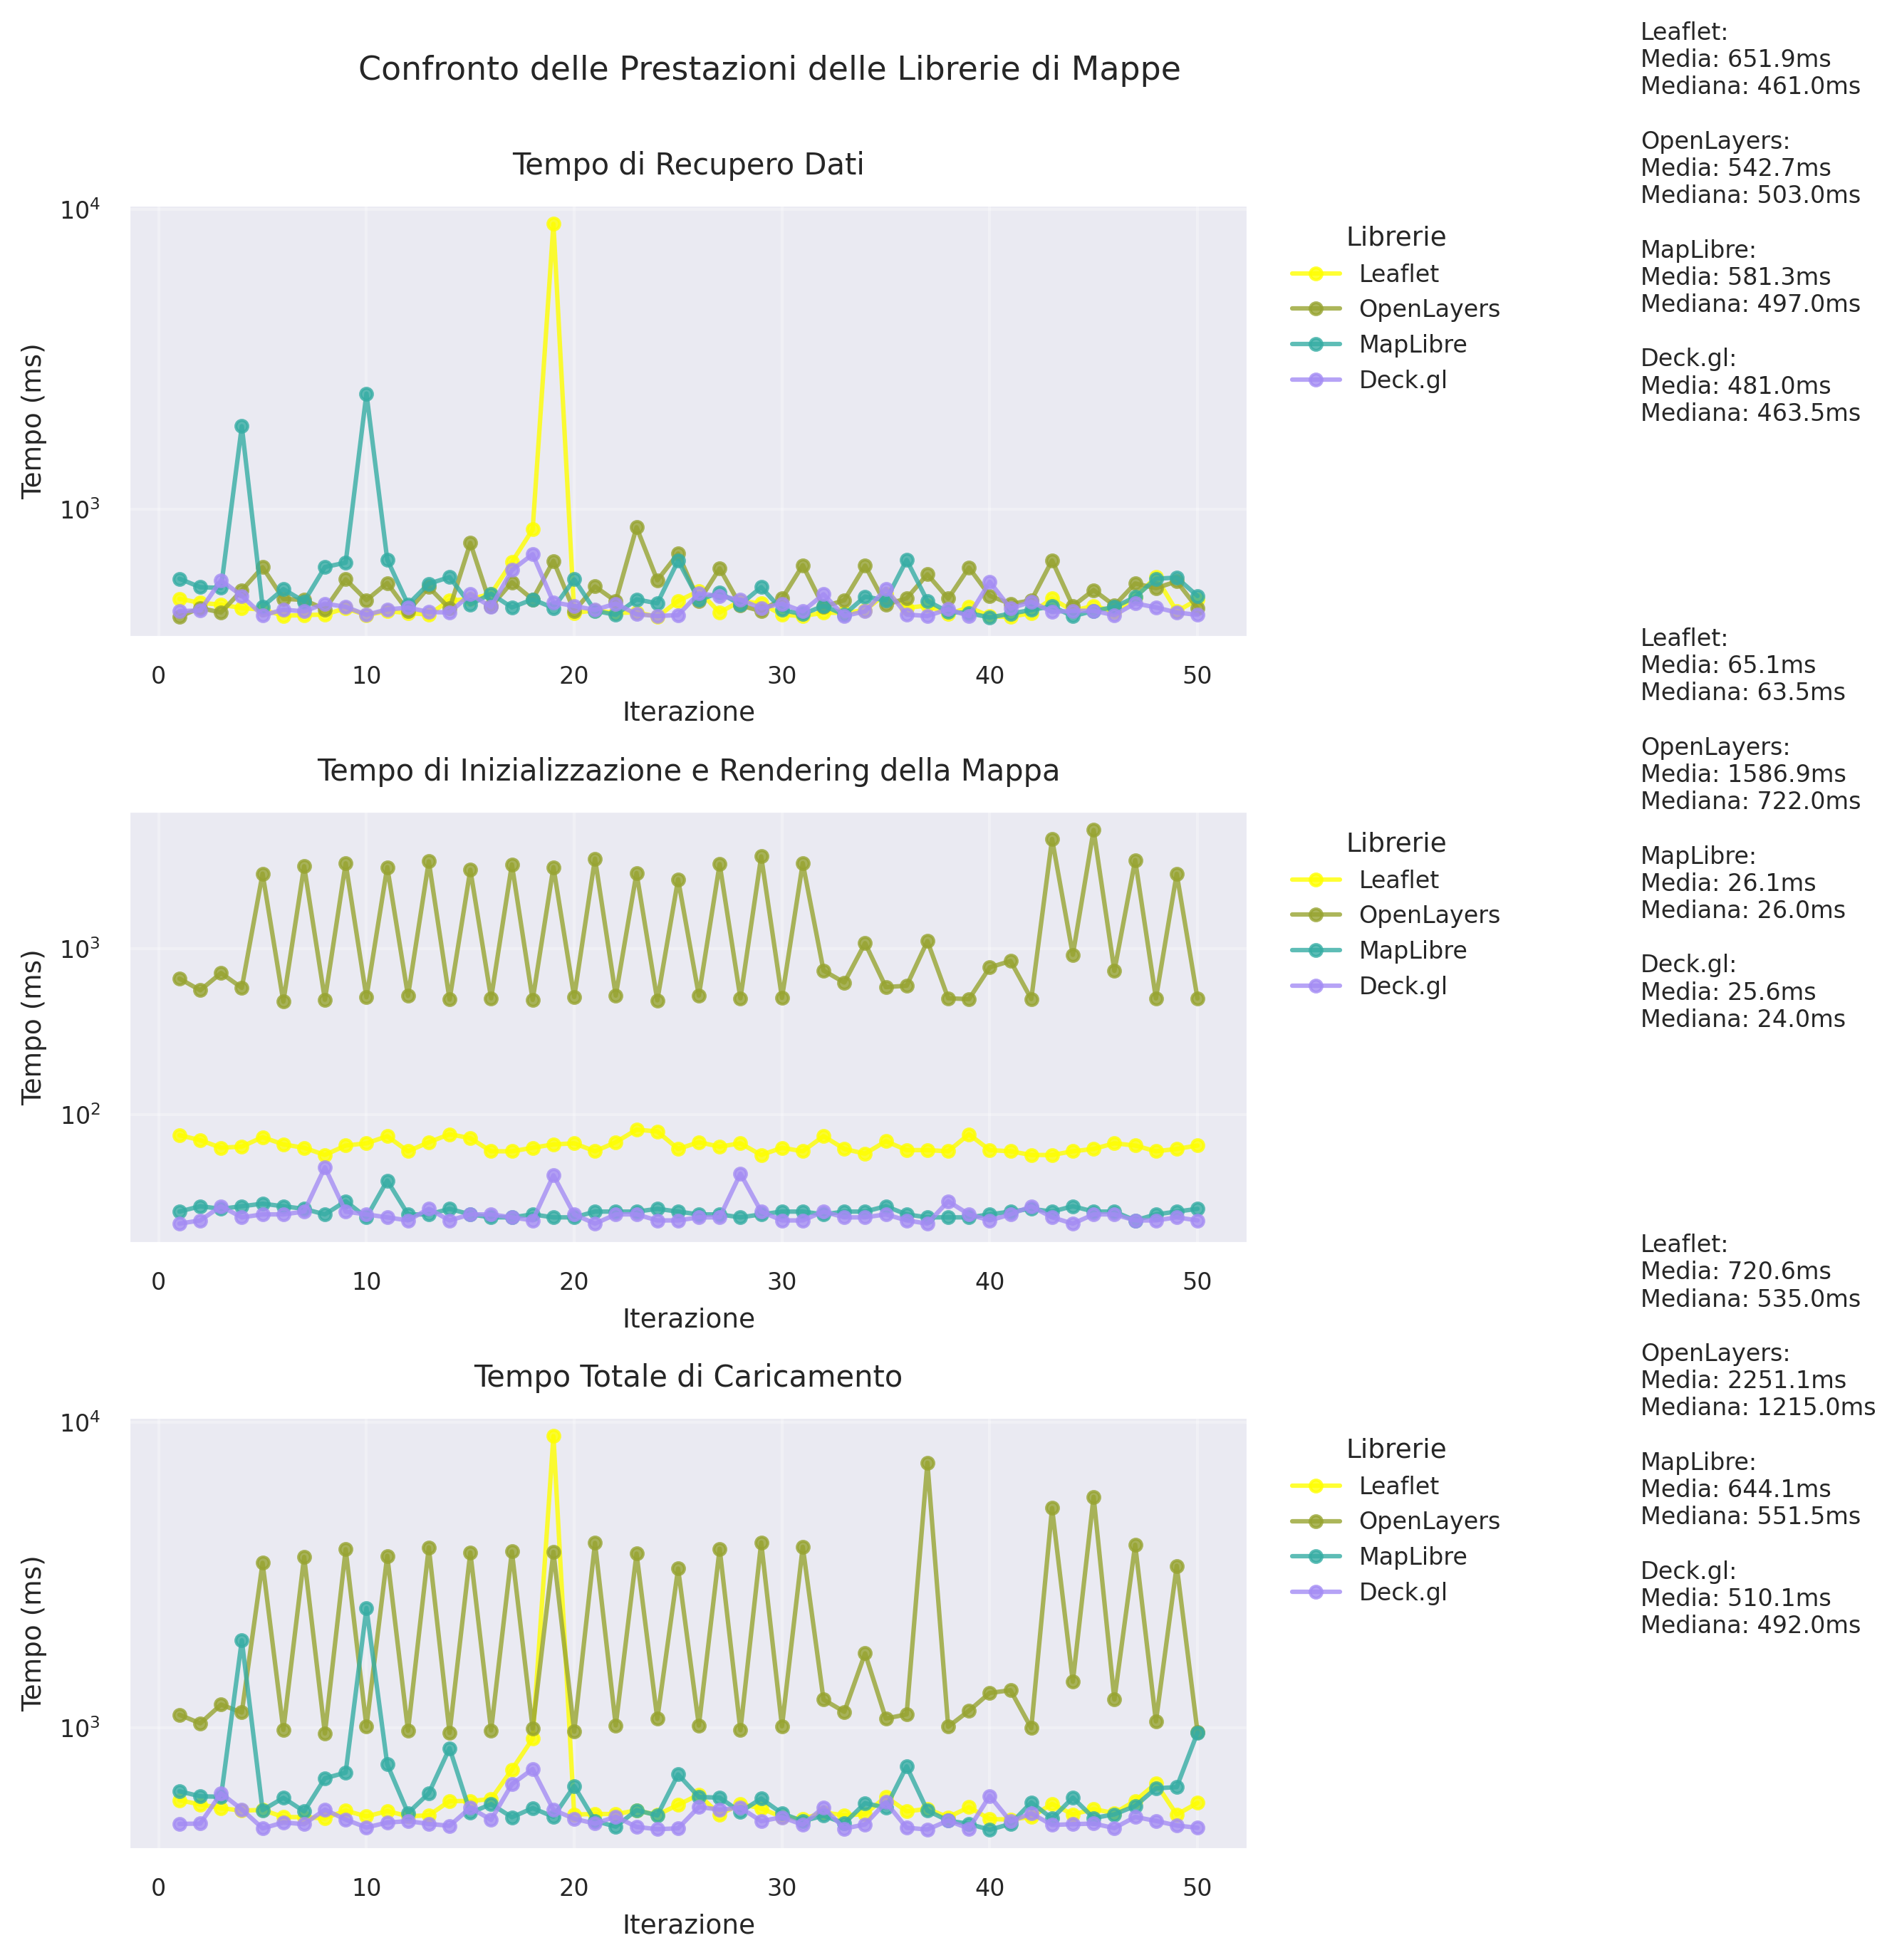
\includegraphics[width=\textwidth]{chapters/librerie-plot/data/confronto_benchmark.png}
    \captionsetup{justification=centering}
    \caption{Grafico combinato di Tempo di caricamento dati,\\ di Inizializzazione Mappa, e Rendering Heatmap}
    \label{fig:map_benchmark}
\end{figure}

\begin{figure}[!ht]
    \centering
    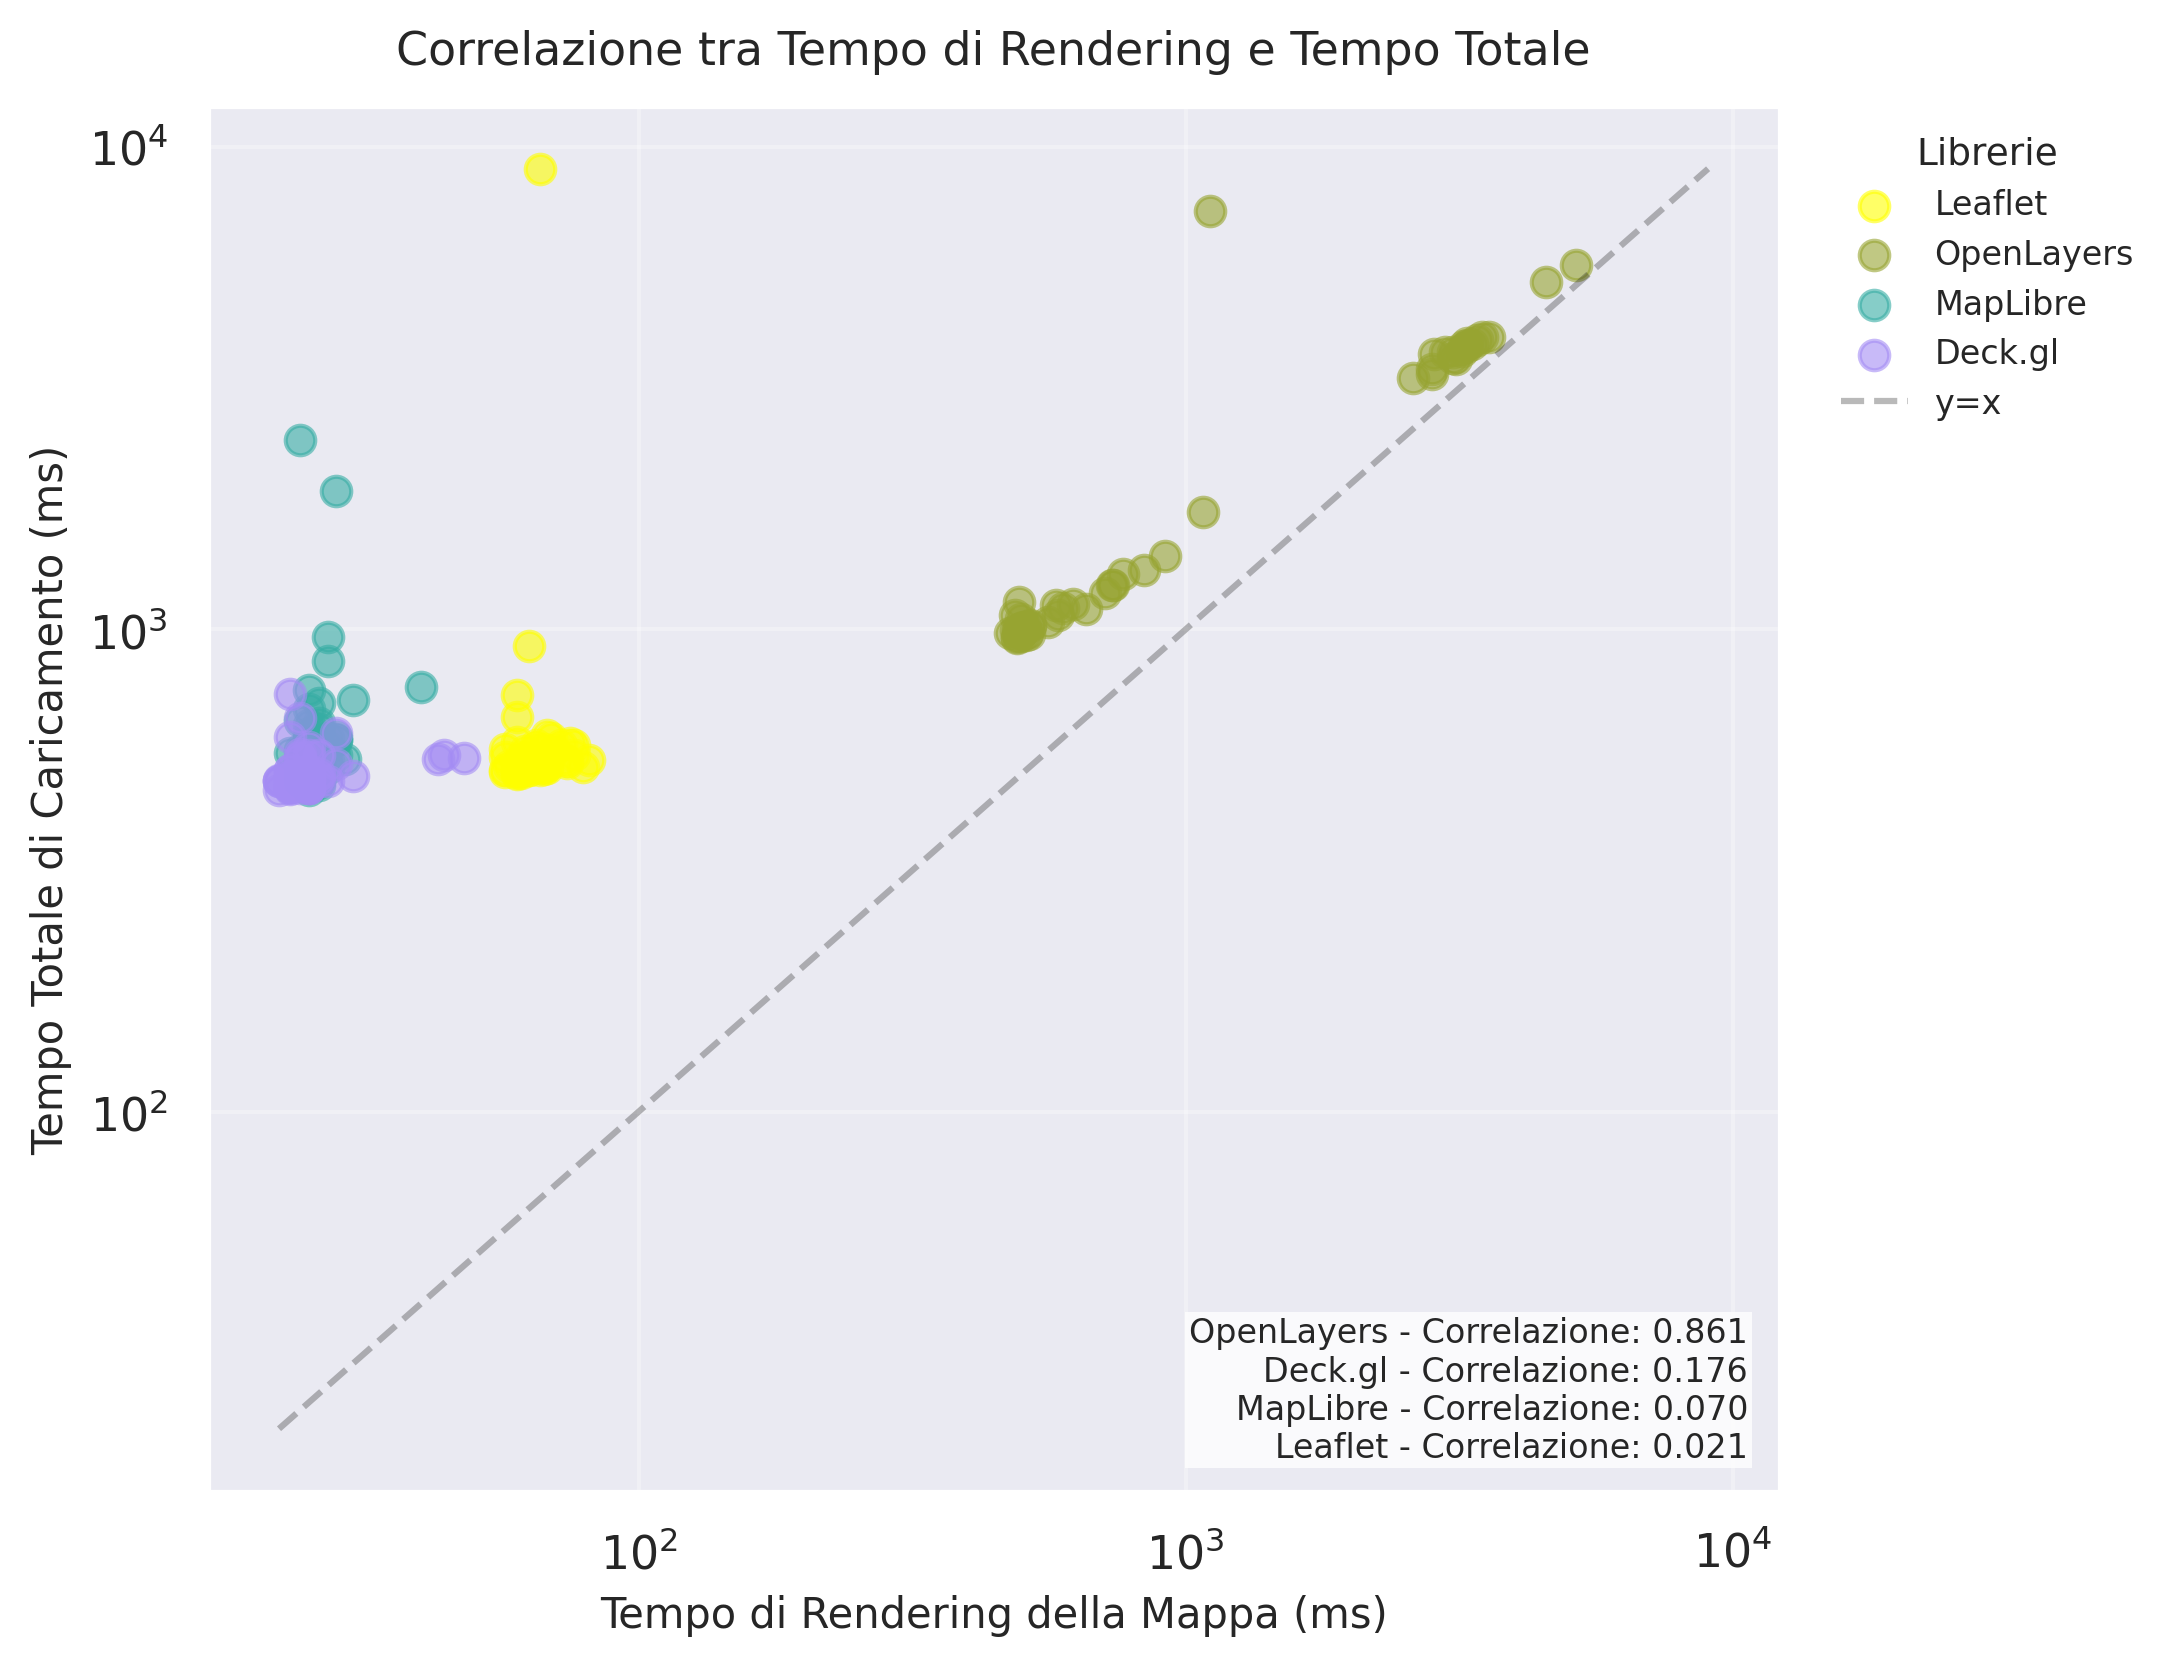
\includegraphics[width=\textwidth]{chapters/librerie-plot/data/correlazione_rendering_totale.png}
    \caption{Grafico che unisce tempo di Inizializzazione Mappa e Rendering Heatmap}
    \label{fig:map_xy_plot}
\end{figure}



% commento grafico linee
Come illustrato in Figura \ref{fig:map_benchmark}, il grafico riassume le prestazioni delle librerie poste in analisi, in relazione alle metriche chiave di caricamento. Le linee presenti nei grafici delineano l'andamento dei dati rilevati e permettono di valutare in modo visivo i punti di forza e di debolezza di ciascuna soluzione.

Nello specifico, il grafico mette a confronto i seguenti dati rilevati:
    \begin{itemize}
        \item Tempo di Recupero dei Dati Geospaziali
        \item Tempo di Inizializzazione e Rendering della Mappa
        \item Tempo totale di Caricamento
    \end{itemize}
    

L'asse \textbf{verticale} rappresenta il tempo in millisecondi impiegato, mentre l'asse \textbf{orizzontale} categorizza la sequenza di rilevazioni ottenute.

Si osserva che le librerie Deck.gl e MapBox/MapLibre eccellono particolarmente nel tempo di inizializzazione e rendering, seguite da Leaflet, registrando i valori più bassi, il che le rende una scelta ottimale per scenari in cui tale aspetto è critico. Al contrario, la libreria OpenLayers mostra prestazioni meno competitive nello stesso ambito, suggerendo aree che richiedono potenziale ottimizzazione o che la rendono meno adatta per carichi di lavoro specifici.

È interessante notare come Leaflet e Deck.gl mostrino prestazioni simili e costantemente basse per il tempo di rendering e OpenLayers presenti una variabilità maggiore per il tempo totale di caricamento. Questo potrebbe indicare fattori architetturali comuni, diverse strategie di ottimizzazione, o impatti di terze parti meno controllabili.

L'analisi di questo grafico di confronto è fondamentale per orientare la scelta della libreria più adatta alle esigenze specifiche del progetto. Essa rivela non solo le performance assolute, ma anche le loro caratteristiche relative, permettendo di identificare la soluzione che meglio si allinea ai requisiti di velocità e reattività dell'applicazione finale.

% commento grafico xy
Ora prendiamo in considerazione ciò che viene illustrato in Figura \ref{fig:map_xy_plot}. Questo  grafico di dispersione presenta la relazione tra il tempo impiegato per il \textbf{rendering della mappa} (misurato in millisecondi sull'asse delle ascisse) e il \textbf{tempo totale di caricamento lato client} (misurato in millisecondi sull'asse delle ordinate). Ogni punto sul grafico rappresenta una singola osservazione di test, e le diverse librerie cartografiche (Leaflet, OpenLayers, MapLibre, Deck.gl), ognuna differenziata da un colore diverso, permettono di distinguere visivamente i loro rispettivi comportamenti.

\begin{itemize}
    \item \textbf{Limite inferiore}
    Si osserva una disposizione dei dati ben definita, dove nessuna libreria è in grado di raggiungere tempi totali di caricamento sotto una certa soglia (indicativamente, $\sim 500$ ms). Interessante la disposizione dei \textit{datapoints} lungo l'asse delle ascisse, quindi l'asse lungo il quale sono disposti i tempi di caricamento in primo luogo della mappa e successivamente del componente \textit{Heatmap}. Ricordo che tale valore è compreso nel più generale tempo di caricamento totale, rappresentato dall'asse delle ordinate; da questo accorgimento si può giustificare l'assenza di \textit{datapoints} situati sotto alla diagonale ipotetica $y=x$.
    
    Le librerie cartografiche che si distinguono per la vicinanza all'origine (Deck.gl, Leaflet, MapLibre) infatti hanno tutte in comune tempi di caricamento dei componenti Mappa e \textit{Heatmap} molto bassi, metrica che può dire la sua nella scelta della libreria per uno specifico caso d'uso.

    \item \textbf{Ulteriori osservazioni}
    Sebbene il grafico in Figura \ref{fig:map_xy_plot} faccia intendere quali siano le librerie generalmente più rapide, è da riconoscere anche un'ulteriore caratteristica: Il grado di correlazione tra i due valori misurati (Tempo di rendering della Mappa e Tempo Totale di Caricamento). Librerie collocate vicino alla diagonale immaginaria $y=x$ sono caratterizzate quindi da una minor differenza tra i due valori misurati. Ciò può indicare un comportamento interessante: in questo caso specifico, abbiamo una libreria (OpenLayers) che impiega più tempo delle altre per il rendering della mappa, ma il tempo di caricamento totale lato \textit{client} risulta poco superiore; questo potrebbe indicare una peggior ottimizzazione lato \textit{Heatmap}, per cui il rendering di tale elemento rappresenta la maggior parte del tempo impiegato dalla libreria per mostrare la mappa a schermo. Un miglioramento su tale versante porterebbe i \textit{datapoints} di tale libreria in una zona più bassa del grafico, probabilmente poco distante dalla diagonale immaginaria. Oppure, adottando una prospettiva più diretta, la libreria nella sua interezza non è tra le più rapide, con o senza \textit{Heatmap}.
    Ed è proprio per via di questa variabilità nell'interpretazione di tale comportamento che i dati riportati in questo grafico risultano utili solamente nell'individuare la libreria generalmente più veloce; è solo dopo aver visivamente accantonato le librerie con tempo totale più elevato delle altre che si è in grado di apprezzare la metrica che valuta il tempo di caricamento della mappa e del componente \textit{Heatmap}.
          
\end{itemize}

In sintesi, l'analisi di questo grafico di correlazione fornisce \textit{insight} preziosi dati sulla dipendenza del tempo di caricamento totale dalle performance di rendering.

\subsection*{Considerazioni sulla Validità e Interpretazione dei Risultati}
È fondamentale sottolineare che, nonostante gli sforzi per standardizzare il processo, le misurazioni di performance nel contesto di un browser web sono intrinsecamente soggette a una certa variabilità. Fattori quali il carico di sistema della macchina ospite, l'attività di altri processi, le specifiche estensioni del browser installate e le fluttuazioni nella latenza di rete (per il recupero di tile e dati) possono influenzare i risultati.
Le specifiche del sistema sul quale sono state effettuate le misurazioni sono brevemente riportate nel frammento di codice nel Listing \ref{lst:inxi_output}.

\begin{listing}[H]
\caption{Output del comando \texttt{inxi}}
\label{lst:inxi_output}
\begin{minted}{bash}
$ inxi
CPU: 8-core AMD Ryzen 7 5800X (-MT MCP-) speed/min/max: 3384/556/4854 MHz
Kernel: 6.15.2-arch1-1 x86_64 Up: 2h 13m Mem: 8.44/15.52 GiB (54.4%)
Storage: 1.6 TiB (30.9% used) Procs: 403 Shell: Bash inxi: 3.3.38
\end{minted}
\end{listing}